\documentclass[14pt]{extarticle}
\usepackage{mathtext}
\usepackage[T2A]{fontenc}
\usepackage[utf8]{inputenc}
\usepackage[russian]{babel}
\usepackage{amsmath}
\usepackage{amsfonts}
\usepackage{amssymb}
\usepackage{graphicx}
\usepackage[top=20mm, bottom=20mm, left=30mm, right=15mm]{geometry}
\usepackage{color}
\usepackage{gensymb}
\usepackage{wrapfig}
\usepackage{float}
\usepackage{longtable}

\usepackage{enumitem}
\setlist[enumerate]{label*=\arabic*.}

\usepackage{indentfirst}

\usepackage{titlesec}
\newcommand{\sectionbreak}{\clearpage}
\renewcommand{\baselinestretch}{1.5}

\graphicspath{ {/home/artem/Documents/University/Research/Report/images/} }

\begin{document}
\begin{titlepage}	% Титульник
	\begin{center}
	{ Федеральное государственное бюджетное образовательное учреждеие высшего профессионального образования \\}
	\end{center}


   \begin{minipage}{0.80\textwidth}
		\begin{large}
			\begin{center}
				{
		\textbf{<<Московский государственый технический университет \\ имени Н.Э. Баумана>> \\ (МГТУ им. Н.Э. Баумана) \\}
   				}
			\end{center}
   		\end{large}
	\end{minipage}

   \begin{center}
    \vspace{0.25cm}
	\noindent\makebox[\linewidth]{\rule{\textwidth}{0.4pt}}

    ФАКУЛЬТЕТ "Энергомашиностроение"

    КАФЕДРА Э-3 "Газотурбинные и нетрадиционные энергоустановки"
    \vspace{1cm}


    \begin{large}\textbf{КУРСОВАЯ НАУЧНО-ИССЛЕДОВАТЕЛЬСКАЯ РАБОТА СТУДЕНТА}\end{large}

	\end{center}
    \textbf{на тему:} Применение нейронных сетей для моделирования подсеточных напряжений при использовании метода больших вихрей

    \textbf{группа:} Э3-101

    \begin{small}\textbf{Выполнил(а) студент(ка)} \makebox[9cm]{\hrulefill}  \textbf{А.Клюквин} \\
    \centerline{(подпись, дата)}
    \end{small}

    \begin{small}\textbf{Руководитель} \makebox[11.8cm]{\hrulefill}   \textbf{С.Бурцев} \\
    \centerline{(подпись, дата)}
    \end{small}



\vfill

\begin{center}
  Москва - 2017 г.
\end{center}
\end{titlepage}


\subsection{Используемые обозначения}
\begin{itemize}
    \item[] $\alpha$ - коэффициент избытка воздуха;
    \item[] $C_{pв}$, Дж/(кг К) - теплоемкость воздуха;
    \item[] $C_{pг}$, Дж/(кг К) - теплоемкость продуктов сгорания природного газа;
    \item[] $C_{pm}$, Дж/(кг К) - теплоемкость топлива;
    \item[] $c_{m.a}$, м/с - осевая скорость на выходе из турбины;
    \item[] $C_e$, Вт/ч - экономичность ГТД;
    \item[] $\eta_k$ - адиабатический КПД компрессора;
    \item[] $\eta_м$ - механический КПД турбины компрессора;
    \item[] $\eta_{тк}$ - адиабатический КПД турбины компрессора;
    \item[] $\eta_р$ - КПД регенератора;
    \item[] $\eta_m$ - адиабатический КПД свободной турбины;
    \item[] $F_m, м^2$ - площадь на выходе из турбины;
    \item[] $g_m$ - удельный расход топлива;
    \item[] $g_т$ - удельный расход газа через турбину;
    \item[] $g_{ут}$ - удельный расход утечек;
    \item[] $g_{охл}$ - удельный расход воздуха на охлаждение;
    \item[] $G_m$, кг/с - расход топлива;
    \item[] $k_г$ - показатель адиабаты продуктов сгорания природного газа;
    \item[] $k_в$ - показатель адиабаты воздуха;
    \item[] $l_0$, кг - масса воздуха, необходимая для сжигания 1 кг топлива;
    \item[] $l_m$, м - длина лопатки на выходе из турбиы;
    \item[] $L_к$, Вт/кг - удельная работа компрессора;
    \item[] $L_{тк}$, Вт/кг - удельная работа турбины компрессора;
    \item[] $L_т$, Вт/кг - удельная работа силовой турбины;
    \item[] $n_т$, об/мин - частота вращения ротора турбины компрессора;
    \item[] $N_{e уд}$, Вт/кг - удельная мощность ГТД;
    \item[] $N_e$, Вт - мощность ГТД;
    \item[] $p_a$, Па - атмосферное давление;
    \item[] $p_ф$, Па - давление за входным фильтром;
    \item[] $p_вх$, Па - давление перед помпрессором;
    \item[] $p_к$, Па - давление за компрессором;
    \item[] $p_{р.х.}$, Па - давление за регенератором по холодной стороне;
    \item[] $p_г$, Па - давление перед турбиной компрессора;
    \item[] $p_{тк}$, Па - давление после турбиные компрессора;
    \item[] $p_с$, Па - давление перед силовой турбиной;
    \item[] $p_т$, Па - давление за силовой турбиной;
    \item[] $p_{р.г.}$, Па - давление за регенератором по горячей стороне;
    \item[] $\pi_к$ - степень повышения давления в компрессоре;
    \item[] $\rho_т, кг/м^3$ - плотность газа на выходе из турбины;
    \item[] $Q_н^р$, Дж/кг - низшая теплота сгорания топлива;
    \item[] $\sigma$ - коэффициент регенерации;
    \item[] $\sigma_г$ - коэффициент сохранения полного давления в камере сгорания;
    \item[] $\sigma_ф$ - коэффициент сохранения полного давления входного фильтра;
    \item[] $\sigma_{вх}$ - коэффициент сохранения полного давления входного устройства компрессора;
    \item[] $\sigma_{р.х.}$ - коэффициент сохранения полного давления по холодной стороне регенератора;
    \item[] $\sigma_{тк}$ - коэффициент сохранения полного давления в патрубке после турбины компрессора;
    \item[] $\sigma_{р.г.}$ - коэффициент сохранения полного давления по горячей стороне регенератора;
    \item[] $\sigma_т$ - коэффициент сохранения полного давления в патрубке за силовой турбиной;
    \item[] $\sigma_{вых}$ - коэффициент сохранения полного давления в выходном устройстве;
    \item[] $T_a$, К - температура атмосферного воздуха;
    \item[] $T_к$, К - температура воздуха за компрессором;
    \item[] $T_р$, К - температура воздуха за регенератором по холодной стороне;
    \item[] $T_г$, К - температура газа перед турбиной;
    \item[] $T_0$, К - температура, при которой определяются теплоемкости веществ;
    \item[] $T_{тк}$, К - температура газа за турбиной компрессора;
    \item[] $T_т$, К - температура газа за силовой турбиной;
    \item[] $u_т$, м/с - окружная скорость на выходе из турбины;
\end{itemize}
%\input{input_data}
\subsection{Расчет цикла}
В данном расчете учет изменения теплофизических свойств рабочего тела в зависимости от его температуры производился
путем итерирования на каждом этапе расчета до тех пор, пока изменение искомого теплофизического свойства (теплоемкости или
показателя адиабаты) не составляло менее 0.1\% в сравнении с результатами предыдущей итерации. Ниже везде используются
значения теплофизический свойств на последнем этапе итерационных расчетов.

\begin{enumerate}
	\item Определим давление за входным устройством:
		$$p_{вх}^* = \sigma_{вх}  p_a = 0,98 \cdot 0,100 = 0,098 \/\ МПа$$
	\item Определим давление за КНД:
		$$p_{кнд}^* = \pi_{кнд} p_{вх}^* = 4,8 \cdot 0,098 = 0,466 \/\ МПа$$
	\item Определим адиабатический КПД КНД $\eta_{кнд}$, принимая показатель адиабаты воздуха $k_{в \/\ кнд} = 1,40$:
	    $$
	    	\eta_{кнд} = \frac{
		        \pi_{кнд}^\frac{
		            k_{в \/\ кнд} - 1
		        }{
		            k_{в \/\ кнд}
	            } - 1
		    }{
		        \pi_{кнд}^\frac{
		            k_{в \/\ кнд} - 1
	            }{
	                k_{в \/\ кнд} \cdot \eta_{пол \/\ кнд}
	            } - 1
		    } = \frac{
	            4,8^\frac{
	                1,40 - 1
	            }{
	                1,40
	            } - 1
	        }{
	            4,8^\frac{
	                1,40 - 1
	            }{
	                1,40 \cdot 0,840
	            } - 1
	        } = 0,80
	    $$
	\item Определим температуру газа за КНД:
		$$T_{КНД}^* = T_a 
		\left[ 
			1 + \frac{
				\pi_к^{
					\frac{
						k_{в \/\ кнд} - 1
					}{
						k_{в \/\ кнд}
					}
				} - 1
			}{
				\eta_{кнд}
			}
		\right] =
			288,0 
		\left[
			1 + \frac{
				{4,8}^{
					\frac{
						1,40 - 1
					}{
						1,40
					}
				} - 1
			}{
				0,80
			}
		\right] = 490,0 \/\ К$$
	\item Используя найденный показатель адиабаты воздуха, определим теплоемкость воздуха в процессе сжатия воздуха в КНД:
		$$c_{pв \/\ кнд} = \frac{
			k_{в \/\ кнд}
		}{
			k_{в \/\ кнд} - 1
		} R_в = \frac{
			1,40
		}{
			1,40 - 1
		} \cdot 287,0 = 1012,1 \/\ Дж/(кг \cdot К)$$
	\item Определим работу КНД:
		$$L_{КНД} = c_{pв \/\ кнд} \left( T_{кнд}^* - T_a \right) =
			1012,1 \cdot \left(490,0 - 288,0\right) =
			0,204 \cdot 10^6 \/\ Дж/кг $$
	\item Определим давление перед КВД:
		$$p_{0 \/\ квд}^* = \sigma_{кнд} p_{кнд}^* = 0,98 \cdot 0,466 = 0,456 \/\ МПа$$
	\item Определим давление за КВД:
		$$ p_{квд}^* = \pi_{квд} p_{0 \/\ квд}^* = 4,0 \cdot 0,456 = 1,825 \/\ МПа $$
	\item Определим адиабатический КПД КВД $\eta_{квд}$, принимая показатель адиабаты воздуха $k_{в \/\ КВД} = 1,37$:
	    $$
	    	\eta_{квд} = \frac{
		        \pi_{квд}^\frac{
		            k_{в \/\ квд} - 1
		        }{
		            k_{в \/\ квд}
	            } - 1
		    }{
		        \pi_{кнд}^\frac{
		            k_{в \/\ квд} - 1
	            }{
	                k_{в \/\ квд} \cdot \eta_{пол \/\ квд}
	            } - 1
		    } = \frac{
	            4,0^\frac{
	                1,37 - 1
	            }{
	                1,37
	            } - 1
	        }{
	            4,0^\frac{
	                1,37 - 1
	            }{
	                1,37 \cdot 0,820
	            } - 1
	        } = 0,78
	    $$
	\item Определим температуру газа за КВД:
		$$T_{квд}^* = T_{кнд}^*
		\left[ 
			1 + \frac{
				\pi_к^{
					\frac{
						k_в - 1
					}{
						k_в
					}
				} - 1
			}{
				\eta_{квд}
			}
		\right] =
			490,0 
		\left[
			1 + \frac{
				{4,0}^{
					\frac{
						1,37 - 1
					}{
						1,37
					}
				} - 1
			}{
				0,78
			}
		\right] = 784,3 \/\ К$$
	\item Используя найденный показатель адиабаты воздуха, определим теплоемкость воздуха в процессе сжатия воздуха в КВД:
		$$c_{pв \/\ квд} = \frac{
			k_{в \/\ квд}
		}{
			k_{в \/\ квд} - 1
		} R_в = \frac{
			1,37
		}{
			1,37 - 1
		} \cdot 287,0 = 1061,8 \/\ Дж/(кг \cdot К)$$
	\item Определим работу КВД:
		$$L_{квд} = c_{pв \/\ квд} \left( T_{квд}^* - T_{кнд}^* \right) =
			1061,8 \cdot \left(784,3 - 490,0\right) =
			0,313 \cdot 10^6 \/\ Дж/кг $$
	\item Температура газа за камерой сгорания:
		$$T_г^* = 1450 \/\ К$$
	\item Определим относительный расход топлива. Расчет носит итерационный характер. Ниже описана последняя итерация. Теплоемкость продуктов сгорания природного газа рассчитывается через показатель адиабаты и газовую постоянную газа. При этом газовая постоянная и истинный показатель адиабаты рассчитываются как средневзвешенное соответственных характеристик компонентов продуктов. При расчета приняты следующие значения:
	\begin{enumerate} % список значений для расчета удельного расхода топлива
		\item[1)] теплоемкость топлива:
			$$c_{pm} = 2226,0 \/\ Дж / (кг \cdot К);$$
		\item[2)] температура подачи топлива:
			$$T_m = 300,0 \/\ К;$$
		\item[3)] температура определения теплофизических параметров веществ:
			$$T_0 = 300,0 \/\ К;$$
		\item[4)] истинная теплоемкость воздуха перед камерой сгорания:
			$$c_{pв \/\ г}\left( T_{КВД} \right) = 1095,4 \/\ Дж/(кг \cdot К);$$
		\item[5)] истинная теплоемкость воздуха при температуре определения теплофизических параметров веществ:
			$$c_{pв \/\ г}\left( T_0 \right) = 1002,7 \/\ Дж/(кг \cdot К);$$
		\item[6)] низшая теплота сгорания топлива:
			$$Q_н^р = 49030 \cdot 10^3 \/\ Дж / кг;$$
		\item[7)] полнота сгорания:
			$$\eta_г = 0,98;$$
		\item[8)] масса воздуха, необходимая для сжигания 1 кг топлива:
			$$l_0 = 17,3 \/\ кг;$$
	\end{enumerate}
	
	\begin{enumerate}
		\item Зададимся коэффициентом избытка воздуха: $$\alpha = 3,32;$$
		\item Теплоемкость продуктов сгорания природного газа $c_{pг \/\ г}$ при данном значении коэффициента избытка воздуха при температуре $T_г$ составляет:
			$$c_{pг \/\ г}\left( T_г \right) = 1222,3 \/\ Дж/(кг \cdot К);$$
		\item Теплоемкость продуктов сгорания природного газа $c_{pг \/\ г}$ при данном значении коэффициента избытка воздуха при температуре $T_0$ составляет:
			$$c_{pг \/\ г}\left( T_0 \right) = 995,0 \/\ Дж / (кг \cdot К);$$
		\item Определим относительный расход топлива:
			$$
				a = c_{pг \/\ г} \left( T_г \right) T_г - c_{pв \/\ г} \left( T_{квд} \right) T_{квд} = 
			$$
			$$
				= 1222,3 \cdot 1450,0 -
				1222,3 \cdot 784,310 = 
				0,913 \cdot 10^6 \/\ Дж/кг
			$$
			$$
				b = \left(
					c_{pг \/\ г}\left( T_0 \right) - c_{pв \/\ г}\left( T_0 \right) = 
				\right) T_0 = 
			$$
			$$
				= \left(
					995,0 - 1002,7
				\right) \cdot 300,0 = 
				-2,327 \cdot 10^3 \/\ Дж/кг
			$$
			$$
				c = c_{pг \/\ г} \left( T_г \right) T_г - c_{pг \/\ г} \left( T_0 \right) T_0 = 
			$$
			$$
				= 1222,3 \cdot 1450,0 -
				995,0 \cdot 300,0 = 
				1,474 \cdot 10^6 \/\ Дж/кг
			$$
			$$
				d = c_{pm} \left( T_m - T_0 \right) = 
			$$
			$$
				= 2226,0 \left( 300,0 - 300,0 \right) =
				0 \/\ Дж/кг
			$$
			$$g_m = \frac{G_m}{G_в^г} =
				\frac{
					a - b
				}{
					Q_н^р \eta_г -
					c + d
				} = 
			$$
			$$
				= \frac{
					0,913 \cdot 10^6 + 2,327 \cdot 10^3
				}{
					49030 \cdot 10^3 \cdot 0.98 -
					1473,793 \cdot 10^6 + 0
				} = 0,017
			$$
		\item Определим коэффициент избытка воздуха:
			$$\alpha^\prime = \frac{1}{g_m l_0} =
		\frac{1}{0,017 \cdot 17,3} = 3,32$$
	\end{enumerate}

	\item Определим удельный расход через ТВД:
		$$g_{твд} = \left( 1 + g_m \right) \left( 1 - g_{ут \/\ твд} - g_{охл \/\ твд} \right) = $$
		$$
		= \left(
		    1 + 0,017
		\right) \left(
		    1 - 0,010 -
		    0,100
        \right) = 1,027$$
	\item Определим удельную работу ТВД:
		$$L_{твд} = \frac{L_{квд}}{g_{твд}\eta_{м \/\ вд}} = \frac{
			0,313 \cdot 10^6
		}{
			1,027 \cdot 0,990
		} = 0,280 \cdot 10^6 \/\ Дж/кг$$
	\item Определим давление газа перед ТВД:
		$$p_{г}^* = p_{тнд}^* \sigma_г = 1,825 \cdot 0,99 = 1,807 \/\ МПа$$
	\item Определим среднюю теплоемкость газа в процессе расширения газа в турбине, принимая показатель адиабаты газа $k_{г \/\ твд} = 1,32$:
		$$c_{pг \/\ твд} = \frac{k_{г \/\ твд}}{k_{г \/\ твд} - 1} R_г =
			\frac{
				1,32
			}{
				1,32 - 1
			} \cdot 291,0 = 1206,6 \/\ Дж/(кг \cdot К) $$
	\item Определим давление воздуха за ТВД:
		$$p_{твд}^* = p_г^*
			\left[
				1 - \frac{L_{твд}}{c_{pг \/\ твд} T_г \eta_{твд}}
			\right] ^ \frac{k_{г \/\ твд}}{k_{г \/\ твд} - 1} =
		$$
		$$
			= 1,807
			\left[
				1 - \frac{0,313 \cdot 10^6}
				{1206,6 \cdot 1450,0 \cdot 0,880}
			\right] ^ \frac{1,32}{1,32 - 1} =
			 0,787 \/\ МПа
		$$
	\item Определим температуру газа за ТВД:
	 	$$
	 		T_{твд}^* = T_г^*
			\left\lbrace
			 	1 -
			 	\left[
			 		1 -
			 			\left(
			 				\frac{p_{твд}^*}{p_г^*}
			 			\right) ^ \frac{k_{г \/\ твд}}{k_{г \/\ твд} - 1}
			 	\right] \eta_{ТВД}
			\right\rbrace =
		$$
		$$
			= 1450,0
			\left\lbrace
			 	1 -
			 	\left[
			 		1 -
			 			\left(
			 				\frac{0,787}{1,807}
			 			\right) ^ \frac{1,32}{1,32 - 1}
			 	\right] \cdot 0,880
			\right\rbrace = 1218,1 \/\ К
		$$
	\item Определим давление перед ТНД:
		$$p_{0 \/\ тнд}^* = p_{твд}^*\sigma_{твд} = 0,787 \cdot 0,98 = 0,771 \/\ МПа$$

	\item Определим удельный расход через ТНД:
		 $$g_{тнд} = g_{твд} \left( 1 - g_{ут \/\ тнд} - g_{охл \/\ тнд} + g_{охл \/\ твд}\right) = $$
		 $$=1,027 \cdot
		 	\left(
		 	    1 - 0,010 -
		 	    0,000 +
		 	    0,100
		 	\right) = 1,037$$
	\item Определим удельную работу ТНД:
		$$L_{тнд} = \frac{L_{кнд}}{g_{тнд}\eta_{м \/\ нд}} = \frac{
			0,204 \cdot 10^6
		}{
			1,037 \cdot 0,99
		} = 0,199 \cdot 10^6 \/\ Дж/кг$$
	\item Определим среднюю теплоемкость газа в процессе расширения газа в ТНД, принимая показатель адиабаты газа $k_{г \/\ тнд} = 1,33$:
		$$c_{pг \/\ тнд} = \frac{k_{г \/\ тнд}}{k_{г \/\ тнд} - 1} R_г =
			\frac{
				1,33
			}{
				1,33 - 1
			} \cdot 291,0 = 1178,1 \/\ Дж/(кг \cdot К) $$
	\item Определим давление воздуха за ТНД:
		$$
			p_{тнд}^* = p_{0 \/\ тнд}^*
				\left[
					1 - \frac{L_{тнд}}{c_{pг \/\ тнд} T_г \eta_{тнд}}
				\right] ^ \frac{k_{г \/\ тнд}}{k_{г \/\ тнд} - 1} =
		$$
		$$
			= 0,771
				\left[
					1 - \frac{
						0,204 \cdot 10^6
					}
					{
						1178,1 \cdot 1218,1 \cdot 0,90
					}
				\right] ^ \frac{1,33}{1,33 - 1} =
				 0,391 \/\ МПа
		$$
	\item Определим температуру газа за ТНД:
	 	$$
	 		T_{тнд}^* = T_{твд}^*
			\left\lbrace
			 	1 -
			 	\left[
			 		1 -
			 			\left(
			 				\frac{p_{тнд}^*}{p_{тнд \/\ 0}^*}
			 			\right) ^ \frac{k_{г \/\ тнд}}{k_{г \/\ тнд} - 1}
			 	\right] \eta_{тнд}
			\right\rbrace =
		$$
		$$
			= 1218,1
			\left\lbrace
			 	1 -
			 	\left[
			 		1 -
			 			\left(
			 				\frac{0,391}{0,771}
			 			\right) ^ \frac{1,33}{1,33 - 1}
			 	\right] \cdot 0,90
			\right\rbrace = 1049,1 \/\ К
		$$
	\item Определим давление перед свободной турбиной:
		$$p_{0 \/\ тс}^* = p_{тнд}^*\sigma_{тнд} = 0,391 \cdot 0,98 = 0,384 \/\ МПа$$
	\item Определим удельный расход через силовую турбину:
	    $$g_{тс} = g_{тнд} \left( 1 - g_{ут \/\ тс} - g_{охл \/\ тс} \right) =
            1,037 \cdot
            \left(
                1 - 0,010 -
                0,000
            \right) = 1,027$$
    \item Определим давление торможения на выходе из свободной турбины $p_{тс}^*$:
		$$p_{тс}^* = p_a / \sigma_{вых} = 0,100 \cdot 0,93 = 0,108 \/\ МПа$$
	\item Зададим значение приведенной скорости на выходе из свободной турбины:
		$$\lambda_{вых} = 0,30$$
	\item Определим статическое давление на выходе из свободной турбины, принимая показатель адиабаты газа на выходе из свободной турбины $k_{тс \/\ вых} = 1,36$:
		$$p_{тс} = p_{тс}^* \cdot \pi \left( \lambda_{вых}, \/\ k_{тс \/\ вых} \right)
        =
			0,108
			\cdot \pi \left( 0,30, \/\ 1,36 \right)
        = 0,102 \/\ МПа$$
	\item Определим статическую температуру на выходе из свободной турбины, принимая показатель адиабаты газа $k_{г \/\ тс} = 1,35$::
		$$
			T_{тс} = T_{тнд}^*
			\left\lbrace
			 	1 -
			 	\left[
			 		1 -
			 			\left(
			 				\frac{p_{0 \/\ тс}^*}{p_{тс}}
			 			\right) ^ \frac{k_{г \/\ тс}}{k_{г \/\ тс} - 1}
			 	\right] \eta_{тс}
			\right\rbrace =
		$$
		$$
			= 1049,1
			\left\lbrace
			 	1 -
			 	\left[
			 		1 -
			 			\left(
			 				\frac{
			 					0,384
			 				}{
			 					0,102
			 				}
			 			\right) ^ \frac{1,35}{1,35 - 1}
			 	\right] \cdot 0,92
			\right\rbrace = 769,6 \/\ К
		$$
	\item Определим температуру торможения на выходе из силовой турбины:
		$$T_{тс}^* = 
			\frac{T_{тс}}{\tau\left( \lambda_{вых}, \/\ k_{тс \/\ вых} \right)} =
			\frac{T_{тс}}{\tau\left( 0,30, \/\ 1,36 \right)} =
			= 780,2 \/\ К$$
	\item Определим значение теплоемкости газа в свободной турбине:
		$$c_{p \/\ тс} = 
			\frac{k_{г \/\ тс}}{k_{г \/\ тс} - 1} = 
			\frac{1,35}{1,35 - 1} = 1133,2 \/\ Дж / \left( кг \cdot К \right)$$
	\item Определим удельную работу силовой турбины:
		$$L_{тс} = c_{p \/\ тс} \left( T_{тнд}^* - T_{тс}^* \right) = 
			1133,2 \cdot \left( 1049,1 - 780,2 \right) =
			0,305 \cdot 10^6\/\ Дж/кг$$
	\item Определим удельную работу ГТД:
		$$L = L_{тс} \/\ g_{тс} =
			0,30 \cdot 10^6 \cdot 1,027 =
			0,305 \cdot 10^6 Дж/кг$$
	\item Определим экономичность ГТД:
		$$C_e = \frac{3600}{N_{e уд}} g_{тс} =
			\frac{3600}{0,305 \cdot 10^6} \cdot 1,03 =
			0,192 \cdot 10^{-3} кг/\left( кВт/ч \right)$$
	\item Определим КПД ГТД:
		$$\eta_e = \frac{3600}{C_e Q_н^р} =
			\frac{3600}{0,192 \cdot 10^{-3} \cdot 49,030 }
			= 0,382$$
	\item Определим потребную мощность ГТД:
		$$
			N = N_e / \eta_р = 16000 \cdot 10^3 \cdot \ 0,98 = 16327 \cdot 10^3 \/\ Вт
		$$
	\item Определим расход воздуха:
		$$G_в = \frac{N}{L} =
			\frac{16327 \cdot 10^3}{0,305 \cdot 10^6} =
			51,1 \/\ кг/с$$
\end{enumerate}
\subsection{Поступенчатый расчет турбины}
Для данного проекта выбрана одноступенчатая турбина.
Исходные параметры для поступенчатого расчета турбины приведены в табл. ~\ref{turbine:midline_inlet}.
Расчет проведен по методике ~\cite{gtd_theory_text_book, mikhaltsev_1, mikhaltsev_2}.
\begin{center}
	\begin{longtable}{|p{4cm}|c|c|c|}
		\caption{Исходные параметры поступенчатого расчета турбины}
		\label{turbine:midline_inlet}
		\endfirsthead
		\caption*{\tabcapalign Продолжение таблицы~\thetable}\\[-0.45\onelineskip]
		\hline
		\textbf{Величина} & \textbf{Обозначение} & \textbf{Размерность} & \textbf{Значение} \\ \hline
		\endhead
		\hline
		\textbf{Величина} & \textbf{Обозначение} & \textbf{Размерность} & \textbf{Значение} \\ \hline
			Реактивность ступени & $\rho$ & - & 0,3  \\ \hline
			Радиальный зазор & $\delta_r$ & м & $1,00 \cdot 10^{-3}$ \\ \hline
			Относительная длина лопатки статора & $\left( \frac{l}{D} \right)_1$ & - & $0,107$ \\ \hline
			Удлинение лопатки статора & $\left( \frac{l}{b_a} \right)_{СА}$ & - & $1,70$ \\ \hline
			Удлинение лопатки ротора & $\left( \frac{l}{b_a} \right)_{РК}$ & - & $2,10$ \\ \hline
			Относительная ширина зазора между лопатками ротора и лопатками статора & $\left( \frac{\delta}{b_a} \right)_{СА}$ & - & $0,10$ \\ \hline
			Угол раскрытия на втулке & $\gamma_{в}$ & \degree & $8,0$ \\ \hline
			Угол раскрытия на периферии & $\gamma_{п}$ & \degree & $20,0$ \\ \hline
			Удельная работа турбины & $H_т$ & Дж/кг & $0,341 \cdot 10^6$ \\ \hline
			Коэффициент скорости статора & $\phi$ & - & 0,94 \\ \hline
			Коэффициент скорости ротора & $\psi$ & - & 0,94 \\ \hline
			Направление скорости на выходе из СА & $\alpha_1$ & $\degree$ & 13,0 \\ \hline
			Частота вращения вала турбины & $n$ & $об/мин$ & 12000,0 \\ \hline
	\end{longtable}
\end{center}

Расчет параметров параметров ТВД приведен ниже. Параметры остальных турбин приведены в табл. ~\ref{tab:turbine-stage-total}.
\begin{enumerate}
	\item Определим теплоперепад на сопловом аппарате:
		$$H_с = \left( 1 - \rho \right) H_т =
		\left( 
			1 - 0,3 
		\right) \cdot 0,341 \cdot 10^6 = 
			0,238 \cdot 10^6 \/\ Дж/кг$$
	\item Определим скорость адиабатного истечения из СА:
		$$c_{1 ад} = \sqrt{2 H_с} = 
			\sqrt{2 \cdot 0,238 \cdot 10^6} = 690,5 \/\ м/с$$
	\item Определим скорость действительного истечения из СА:
		$$c_1 = \phi c_{1 ад} =
			0,94 \cdot 690,5 = 651,4 \/\ м/с$$
	\item Определим температуру на выходе из СА:
		$$T_1 = T_г - \frac{c_1^2}{2c_{pг}} =
			1450 - 
			\frac{
				{651,4}^2
			}{
				2 \cdot 1210,3
			} = 1274,7 \/\ К$$
	\item Определим температуру конца адиабатного расширения:
		$$T_1^\prime = T_г - \frac{H_c}{c_{pг}} =
			1450,0 - 
			\frac{
				0,238 \cdot 10^6
			}{
				1210,3
			} = 1255,0 \/\ К$$
	\item Определим давление на выходе из СА:
		$$p_1 = p_г \left( \frac{T_1^\prime}{T_г} \right)^\frac{k_г}{k_г - 1} =
			1,807 \cdot \left(
				 \frac{
				 	1255,0
				 }{
				 	1450,0
				 } 
			\right)^\frac{
				1,32
			}{
				1,32 - 1
			} = 0,991 \/\ МПа$$
	\item Определим плотность газа на выходе из СА:
		$$\rho_1 = \frac{p_1}{R_г T_1} =
			\frac{
				0,991 \cdot 10^6
			}{
				291,0 \cdot 1274,7
			} = 2,67 \/\ кг/м^3$$
	\item Зададим угол на выходе из СА:
		$$\alpha_1 = 13,0 \degree$$
	\item Определим осевую скорость на выходе из СА:
		$$c_{1a} = c_1 \cdot \sin \alpha_1 =
			651,4 \cdot 
			\sin13,0\degree 
			= 146,5 \/\ м/с$$
	\item Определим площадь на выходе из СА:
		$$A_1 = \frac{G}{c_{1a} \rho_1} =
			\frac{
				53,1
			}{
				146,5 \cdot 2,67
			} = 0,13 \/\ м^2$$
	\item Определим средний диаметр турбины на выходе из СА:
	$$D_1 = \sqrt{
		\frac{A_1}{\pi \left( \frac{l}{D} \right)_1}
		} = \sqrt{
			\frac{
				0,13
			}{
				\pi \cdot 0,107
			}
		} = 0,632 \/\ м $$
	\item Определим окружную скорость на среднем диаметре на входе в РК:
		$$u_1 = \frac{\pi D_1 n}{60} = 
			\frac{
				\pi \cdot 0,653 \cdot 12000,0
			}{60} = 398,7 \/\ м/с$$
	\item Определим относительную скорость на входе в РК:
		$$w_1 = \sqrt{c_1^2 + u_1^2 - 2 c_1 u_1 \cos \alpha_1} =$$
		$$
			=\sqrt{
				{651,4}^2 + 
				{398,7}^2 - 
				2 \cdot 651,4 \cdot 398,7 \cdot 
				\cos 13,0 \degree
			} = 277,9 \/\ м/с
		$$
	\item Определим температуру торможения в относительном движении на входе в РК:
		$$T_{w1} = T_1 + \frac{w_1^2}{2c_{p г}} = 
			1274,7 + 
			\frac{
				277,9^2
			}{
				2 \cdot 1194,1
			} = 1306,9 \/\ К$$
	\item Определим давление торможения в относительном движении на входе в РК:
		$$p_{w1} = p_1 \left( \frac{T_{w1}}{T_1} \right)^\frac{k_г}{k_г - 1} =
	 		0,991 \cdot \left( 
	 			\frac{
	 				1306,9
	 			}{
	 				1274,7
	 			} 
	 		\right)^\frac{
	 			1,32
	 		}{
	 			1,32 - 1
	 		} = 1,099 \/\ МПа$$
	 \item Определим теплоперепад на РК:
	 	$$H_л = H_т \rho \frac{T_1}{T_1^\prime} =
	 		0,341 \cdot 10^6 \cdot 0,3 \cdot \frac{
	 			1274,7
	 		}{
	 			1255,0
	 		} = 0,100 \cdot 10^6 \/\ Дж/кг$$
	\item Определим расстояние в осевом направлении между выходными кромками лопаток СА и выходными кромками лопаток РК:
		$$x = \frac{
		 	\frac{\delta_a}{ \left( \frac{l}{b_a} \right)_1 }	+
		 	\frac{1}{\left( \frac{l}{b_a} \right)_2 }
		}{
		 	1 - \frac{\tan \gamma_п + \tan \gamma_в}
		 	{2 \left( \frac{l}{b_a} \right)_2}
		} D_1 \left( \frac{l}{D} \right)_1 =
		\frac{
		 	\frac{
		 		0,10
		 	}{
		 		1,70
		 	}	+
		 	\frac{
		 		1
		 	}{
		 		2,10
		 	} 
		}{
			1 - \frac{
				\tan 20,0 \degree + \tan 8,0 \degree
			}{
				2 \cdot 2,10
			}
		} \cdot 0,632 \cdot 0,107 =
			0,042 \/\ м
		$$
	 \item Определим средний диаметра на выходе из РК:
		 $$D_2 = D_1 + \frac{\tan \gamma_п - \tan \gamma_в}{2} x =
	   		0,632 + 
	   		\frac{
	   			\tan 20,0 \degree - 
	   			\tan 8,0 \degree
	   		}{2} \cdot 0,042 =
   		0,653 \/\ м$$
	 \item Определим длину лопатки на выходе из РК:
		 $$l_2 = 
		 	D_1 \left( \frac{l}{D} \right)_1 + 
		 	\frac{\tan \gamma_п + \tan \gamma_в}{2} x =
	 	$$
	 	$$
	 		= 0,632 \cdot 
		 	0,107 +
		 	\frac{
		 		\tan 20,0 \degree + 
		 		\tan 8,0 \degree
		 	}{2} \cdot 0,042 =
		 		0,078 \/\ м
	 	$$
	 \item Определим относительную длину лопаток на выходе из РК:
		 $$\left( \frac{l}{D} \right)_2 = \frac{l_2}{D_2} = 
		 	\frac{
		 		0,078
		 	}{
		 		0,653
		 	} = 0,120$$
	 \item Определим окружную скорость на среднем диаметре на выходе из РК:
		 $$u_2 = \frac{\pi D_2 n}{60} = 
		 	\frac{
		 		\pi 
		 		\cdot 0,653 
		 		\cdot 12000,0
		 	}{60} = 411,7 \/\ м/с$$
	 \item Определим адиабатическую относительную скорость истечения газа из РК:
	 	$$w_{2 ад} = \sqrt{w_1^2 + 2H_л + \left( u_2^2 - u_1^2 \right)} =$$
	 	$$
	 		= \sqrt{
	 			{277,9}^2 + 
	 			2 \cdot 0,100 \cdot 10^6 + 
	 			\left( {411,7}^2 - {398,7}^2 \right)
	 		} = 535,8 \/\ м/с
	 	$$
	 \item Определим относительную скорость истечения газа из РК:
	 	$$w_2 = \psi w_{2 ад} =
	 		0,94 \cdot 535,8 = 
	 		505,5 \/\ м/с$$
	 \item Определим статическую температуру на выходе из РК:
		 $$
			 T_2 = T_1 + \frac{
			 	\left(
			 		w_1^2  - w_2^2
			 	\right) + \left(
			 		u_2^2 - u_1^2
			 	\right)
			 }{2 c_{p г}} =
		 $$
		 $$
		 	= 1274,7 + \frac{
			 	\left(
			 		{277,9}^2  - {505,5}^2 
			 	\right) + 
			 	\left( 
			 		{398,7}^2  - {411,7}^2
			 	\right)
		 	}{2 \cdot 1194,1} = 
		 		1204,4 \/\ К
		 $$
	 \item Определим статическую температуру при адиабатическом процессе в РК:
		 $$T_2^\prime = T_1 + \frac{
		 	\left(
		 		w_1^2  - w_{2 ад}^2
		 	\right) + 
		 	\left(
		 		u_2^2 - u_1^2
		 	\right)
		 }{2 c_{p г}} =
		$$
		$$
			= 1274,7 + \frac{
			 	\left(
			 		{277,9}^2  - {535,8}^2 
			 	\right) + 
			 	\left( 
			 		{398,7}^2  - {411,7}^2
			 	\right)
			}{2 \cdot 1194,1} = 
			1191,2 \/\ К
		$$
	 \item Определим давление на выходе из РК:
	 	$$p_2 = p_1 
	 		\left( 
	 			\frac{
	 				T_2^\prime
	 			}{
	 				T_1
	 			} 
	 		\right)^{
	 			\frac{
	 				k_г
	 			}{
	 				k_г - 1
	 			}
	 		} =
	 		0,991 
	 		\left( 
	 			\frac{
	 				1191,2
	 			}{
	 				1274,7
	 			} 
	 		\right)^{
	 			\frac{
	 				1,32
	 			}{
	 				1,32 - 1
	 			}
	 		} = 0,751 \/\ МПа$$
	 \item Определим угол в относительном движении на выходе из РК:
	 	$$\beta_2 = \arcsin\frac{c_{2a}}{w_2} = 
	 	\arcsin\frac{
	 		154,6
	 	}{
	 		505,5
	 	} = 17,8 \degree$$
	 \item Определим угол выхода из РК в абсолютном движении:
	 	$$\alpha_2 = \arctan\frac{w_2 \cos \beta_2 - u_2}{c_{2a}} =
	 	\arctan\frac{
	 		505,5 \cdot 
	 		\cos 17,8 \degree - 
	 		411,7
	 	}{
	 		154,6
	 	} = 65,8 \degree$$
	 \item Определим окружную составляющую скорости на выходе из РК:
	 	$$c_{2u} = w_2 \cos \beta_2 - u_2 =
		 	505,5 \cdot 
		 	\cos 17,8 \degree - 
		 	411,7 = 
		 	69,6 \/\ м/с$$
	 \item Определим скорость потока на выходе из РК:
	 	$$c_2 = \sqrt{c_{2u}^2 + c_{2a}^2} = 
	 		\sqrt{
	 			{69,6}^2 + {154,6}^2
	 		} = 169,6 \/\ м/с$$
	 \item Определим степень понижения давления в турбине:
	 	$$\pi_{т} = \frac{p_г}{p_2} = 
	 		\frac{
	 			1,807
	 		}{
	 			0,751
	 		} = 2,41 $$
	 \item Определим осевую составляющую скорости газа за турбиной:
	 	$$c_{2a} = c_2 \sin \alpha_2 = 
	 		169,6 \cdot
	 		\sin 65,8 \degree = 
	 		154,6 \/\ м/с$$
	 \item Определим плотность газа за турбиной:
	 	$$\rho_2 = \frac{G}{\pi \cdot c_{2a} \cdot D_2 \cdot l_2} = 
	 	\frac{
	 		53,1
	 	}{
	 		\pi \cdot 
	 		154,6 \cdot 
	 		0,653 \cdot 
	 		0,078
	 	} = 2,14 \/\ кг/м^3$$
	 \item Определим работу на окружности колеса:
	 $$L_u = c_{1u} u_1 + c_{2u} u_2 = 
	 	146,5 \cdot 398,7 + 
	 	154,6 \cdot 411,7 = 
	 	0,282 \cdot 10^6 \/\ Дж/кг$$
	 \item Определим КПД на окружности колеса:
	 	$$\eta_u = \frac{L_u}{H_t} = 
	 		\frac{
	 			0,282 \cdot 10^6
	 		}{
	 			0,341 \cdot 10^6
	 		} = 0,83 $$
	 \item Определим удельные потери на статоре:
		 $$h_c = \left( \frac{1}{\phi^2} - 1 \right) \frac{c_1^2}{2} =
		 \left( 
		 	\frac{
		 		1
		 	}{
		 		{0,94 }^2
		 	} - 1 
	 	\right) \frac{
	 		{651,4}^2
	 	}{2} = 24,46 \cdot 10^3 \/\ Дж/кг$$
	 \item Определим удельные потери на роторе:
	 	$$h_р = 
	 		\left( 
	 			\frac{1}{\psi^2} - 1 
	 		\right) \frac{w_2^2}{2} =
	 		\left( 
	 			\frac{1}{{0,94}^2} - 1 
	 		\right) \frac{
	 			{505,5}^2
	 		}{2} = 15,76 \cdot 10^3 \/\ Дж/кг$$
	 \item Определим удельные потери с выходной скоростью:
	 	$$h_{вых} = \frac{c_2^2}{2}= 
	 		\frac{
	 			{169,6}^2
	 		}{2} = 14,38 \cdot 10^3 \/\ Дж/кг$$
	 \item Определим удельные потери в радиальном зазоре:
	 	$$h_з = 1.37 \cdot \left( 1 + 1.6 \rho \right)
	 	\left[ 
	 		1 + 
	 		\left( 
	 			\frac{l}{D} 
	 		\right)_1 
	 	\right] \frac{
	 		\delta_r
	 	}{
	 		l_2
	 	} L_u = $$
	 $$ = 1.37 \cdot 
	 	\left( 
	 		1 + 1.6 \cdot 0,3 
	 	\right)
	 	\left[ 
	 		1 + 0,120
	 	\right] \frac{
	 		1,00 \cdot 10^{-3}
	 	}{
	 		0,078
	 	} \cdot 282 \cdot 10^3 =
	 	0,64 \cdot 10^3 \/\ Дж/кг$$
	 \item Определим удельные потери на вентиляцию:
	 	$$h_{вент} = 1.07 D_2^2 \left( \frac{u_2}{100} \right)^3 \rho_2 \cdot 1000 =$$
	 	$$
	 		=1.07 \cdot {0,653}^2 
	 			\left( 
		 			\frac{
		 				411,7
		 			}{
		 				100
		 			} 
	 			\right)^3 
	 			\cdot 2,14 
	 			\cdot 1000 = 1,29 \cdot 10^3 \/\ Дж/кг
	 	$$
	 \item Определим температуру торможения за РК:
	 	$$T_2^* = T_2 + \frac{h_з + h_{вент} + h_{вых}}{c_{pг}} =$$
	 	$$
	 		1204,4 + 
		 	\frac{
		 		0,64 \cdot 10^3 + 
		 		1,29 \cdot 10^3 + 
		 		14,38 \cdot 10^3
		 	}{
		 		1194,1
		 	} = 1218,1 \/\ К
	 	$$
	 \item Определим давление торможения за РК:
	 	$$p_2^* = p_2 
	 		\left( 
	 			\frac{
	 				T_2^*
	 			}{
	 				T_2
	 			} 
	 		\right)^{
	 			\frac{
	 				k_г
	 			}{
	 				k_г - 1
	 			}
	 		} =
	 	0,751 \cdot 
	 		\left( 
	 			\frac{
	 				1218,1
	 			}{
	 				1204,4
	 			} 
	 		\right)^{
	 			\frac{
	 				1,32
	 			}{
	 				1,32 - 1
	 			}
	 		} = 0,787 \/\ МПа$$
	 \item Определим мощностной КПД турбины:
	 	$$\eta_{т \/\ мощн} = 
	 		\eta_u - 
	 		\frac{
	 			h_з + h_{вент}
	 		}{
	 			H_т
	 		} =
	 		0,83 - 
	 		\frac{
	 			0,64 \cdot 10^3 + 1,29 \cdot 10^3
	 		}{
	 			0,341 \cdot 10^6
	 		} = 0,82$$
	 \item Определим работу турбины:
	 	$$L_т = H_т \eta_т = 
	 		0,341 \cdot 10^6 \cdot 
	 		0,82 = 
	 		0,280 \cdot 10^6 \/\ Дж/кг$$
	 \item Определим теплоперепад по параметрам торможения:
	 	$$H_т^* = c_{pг} T_г 
	 		\left[ 
	 			1 - 
	 				\left( 
	 					\frac{
	 						p_2^*
	 					}{
	 						p_г^*
	 					} 
	 				\right)^\frac{
	 					k_г - 1
	 				}{
	 					k_г
	 				} 
	 		\right] =
	 	$$
	 	$$
	 		= 1206,6 \cdot 1450,0 
	 		\left[ 1 - 
	 			\left( 
	 				\frac{
	 					0,787
	 				}{
	 					1,807
	 				} 
	 			\right)^\frac{
	 				1,32 - 1
	 			}{
	 				1,32
	 			} 
	 		\right] = 0,318 \cdot 10^6 \/\ Дж/кг 
	 	$$
	 \item Определим КПД турбины по параметрам торможения:
	 $$\eta_т^* = \frac{L_т}{H_т^*} =
	 	\frac{
	 		0,280 \cdot 10^6
	 	}{
	 		0,318 \cdot 10^6
	 	} = 0,88$$
\end{enumerate}
%\section{Профилирование ступени ТВД}
Исходными данными для данного этапа проектирования турбины являются результы расчета по средней линии тока.

Ступень была спрофилирована по закону $\alpha_1=const$.

Определим треугольники скоростей на произвольном радиусе лопатки.

\begin{enumerate}

	\item В этом случае значения абсолютной скорости на входе на рабочие лопатки на произвольном радиусе определялись по следующим формулам (в приведенных ниже формулах значения со штрихом относятся к среднему радиусу):
		$$
			c_{1u} = c_{1u}^\prime \left( \frac{r^\prime}{r} \right)^{cos^2\alpha}; \/\
			c_{1a} = c_{1a}^\prime \left( \frac{r^\prime}{r} \right)^{cos^2\alpha}; \/\
			c_1 = c_1^\prime \left( \frac{r^\prime}{r} \right)^{cos^2\alpha}
		$$

	\item Окружная скорость рабочей лопатки на произвольном радиусе была определена по закону вращения твердого тела:
		$$
			u = u^\prime \frac{r}{r^\prime}
		$$

	\item Относительная скорость на произвольном радиусе на входе в рабочие лопатки была определена по следующим формулам:
		$$
			w_{1u} = c_{1u} - u; \/\ 
			w_{1a} = c_{1a}; \/\ 
			w_1 = \sqrt{w_{1u}^2 + w_{1a}^2}
		$$

	\item Абсолютная скорость на выходе из рабочих лопаток была определена по условию постоянства работы, отводимой от газа на различных радиусах лопатки.

	По формуле Эйлера для правила отсчета углов, принятого в теории турбин удельная работа на окружности колеса $L_u$ определяется слеюущей формулой:
		$$
			L_u = c_{1u} + c_{2u}
		$$
	Таким образом, зная работу на окружности колеса на среднем радиусе лопатки $L_u^\prime$, мы можем определить значение окружной скорости на выходе из рабочих лопаток:
		$$
			c_{2u} = \frac{L_u^\prime}{u} - c_{1u} =
				\frac{L_u^\prime}{u^\prime} 
				\frac{r^\prime}{r} - 
				c_{1u}^\prime \left( 
					\frac{r^\prime}{r} 
				\right)^{cos^2\alpha_1} 
		$$

	\item Используя значения окружной и осевой скорости на среднем радиусе лопатки, определим значение осевой скорости на выходе из рабочих лопаток, проинтегрировав уравнение радиального равновесия:
		$$
			c_{2a}^2 = c_{2a}^{\prime 2} + c_{2u}^{\prime 2} - c_{2u}^{2} - 2 \int_{r^\prime}^r \frac{c_{2u}^2}{r} dr
		$$
%	Введем обозначения $a = \frac{L_u^\prime}{u}; \/\ b = c_{1u}^\prime$.
%
%	Тогда после интегрирования получим:
%		$$
%			c_{2a} = c_{2a}^{\prime 2} + c_{2u}^{\prime 2} - c_{2u}^{2} +
%			\left. \left[
%				- a^2 \left(
%					\frac{r^\prime}{r}
%				\right)^{2} +
%				\frac{4ab}{
%					1 + cos^2 \alpha_1
%				}\left(
%					\frac{r^\prime}{r}
%				\right)^{1 + \cos^2\alpha_1} -
%				\frac{b^2}{\cos^2 \alpha_1} \left(
%					\frac{r^\prime}{r}
%				\right)^{2cos^2 \alpha_1}
%			\right] \right|_{r^\prime}^r
%		$$

	\item Значения проекций относительной скорости на выходе из лопаток находим так же, как и значения на входе в рабочие лопатки.

%	Определим профили давления и реактивности на произвольном радиусе лопатки:
%	\begin{enumerate}
%		\item Запишем выражение для числа Маха на произвольном радиусе лопатки:
%		$$
%			M_{1, 2} = \frac{
%				c_{1,2}
%			}{
%				\sqrt{kR \left( T_{1, 2} + \frac{{c_{1,2}}^2 - {c_{1,2}^\prime}^2}{c_p} \right)}
%			}
%		$$
%		\item Запишем выражение для давления на произвольном радиусе лопатки, используя ГДФ давления:
%		$$
%			p_{1,2} = p_{1,2}^\prime \frac{
%				\pi(M_{1,2}^\prime), k
%			}{
%				\pi(M_{1,2}), k
%			}
%		$$
%		\item Запишем выражение для статической температура на произвольном радиусе лопатки, используя ГДФ давления:
%		$$
%			p_{1,2} = p_{1,2}^\prime \frac{
%				\pi(M_{1,2}^\prime), k
%			}{
%				\pi(M_{1,2}), k
%			}
%		$$
%	\end{enumerate}

\end{enumerate}

Распределение углов на входе в рабочие лопатки турбины и на выходе из них представлено на рис. 2 и 3, соответственно:
	\begin{figure}[H]
		\centering
		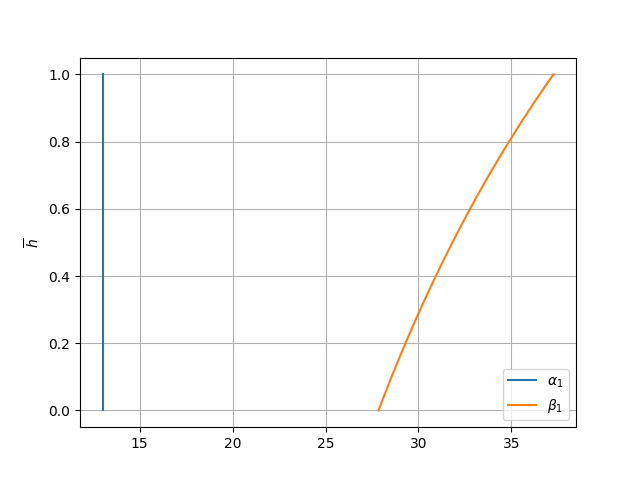
\includegraphics[scale=0.6]{inlet_angle}
		\caption{Углы на входе в лопатки турбины}
	\end{figure}

	\begin{figure}[H]
		\centering
		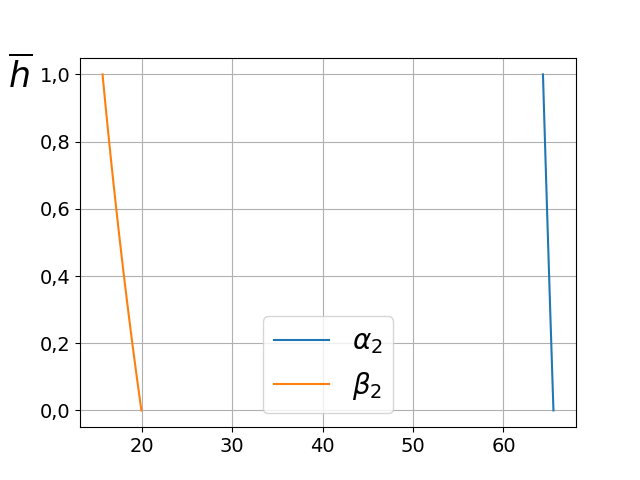
\includegraphics[scale=0.6]{outlet_angle}
		\caption{Углы на выходе из лопаток турбины}
	\end{figure}

%Ниже представлены профили лопаток статора и ротора на трех радиусах
%    \begin{figure}
%        \centering
%        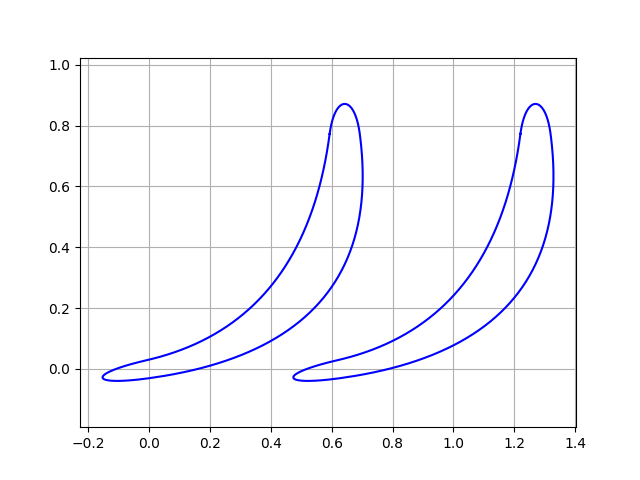
\includegraphics[scale=0.6]{stator_root}
%        \caption{Профиль статора на втулке}
%    \end{figure}
%
%    \begin{figure}
%        \centering
%        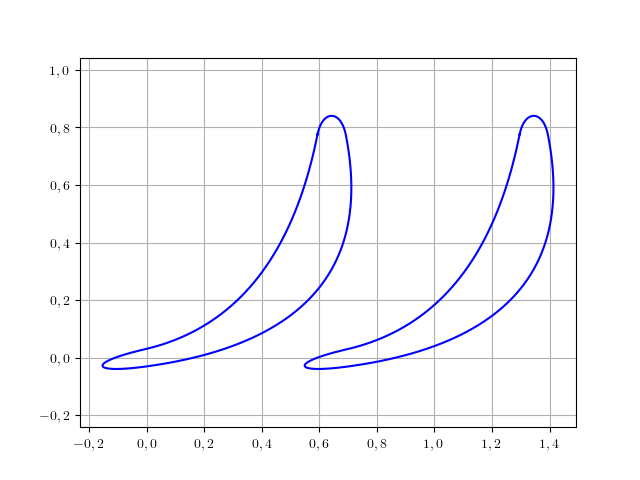
\includegraphics[scale=0.6]{stator_mid}
%        \caption{Профиль статора на среднем радиусе}
%    \end{figure}
%
%    \begin{figure}
%        \centering
%        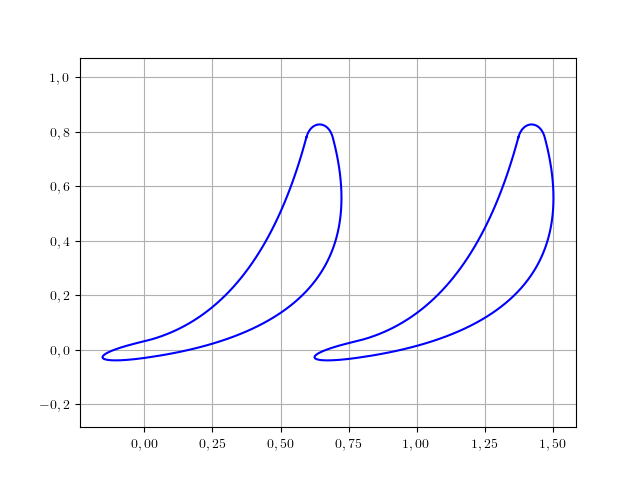
\includegraphics[scale=0.6]{stator_top}
%        \caption{Профиль статора на периферии}
%    \end{figure}
%
%    \begin{figure}
%        \centering
%        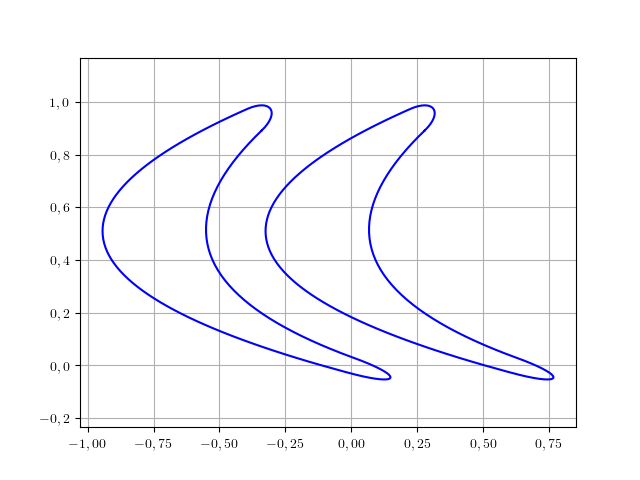
\includegraphics[scale=0.6]{rotor_root}
%        \caption{Профиль ротора на втулке}
%    \end{figure}
%
%    \begin{figure}
%        \centering
%        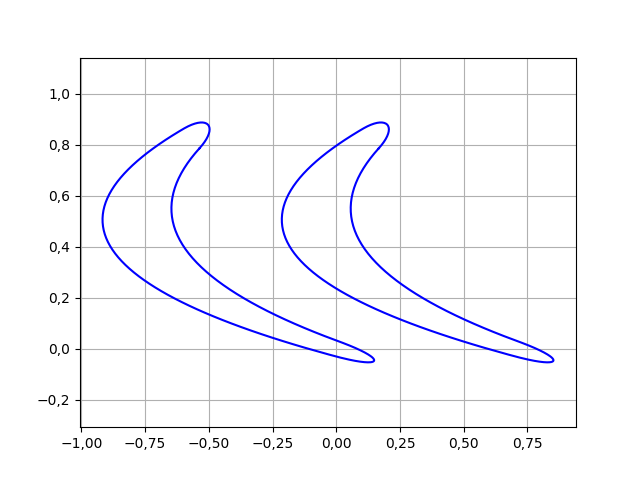
\includegraphics[scale=0.6]{rotor_mid}
%        \caption{Профиль ротора на среднем радиусе}
%    \end{figure}
%
%    \begin{figure}
%        \centering
%        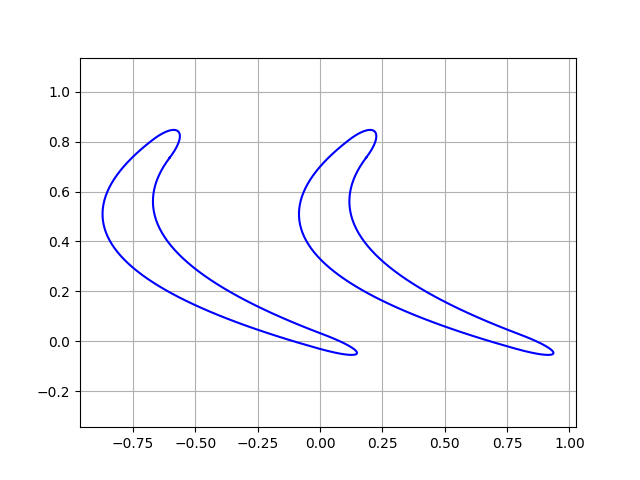
\includegraphics[scale=0.6]{rotor_top}
%        \caption{Профиль ротора на периферии}
%    \end{figure}

%\input{cooling_calc}
%\section{Расчет профиля температур}

Для расчета профиля температур лопатки принимаем расход воздуха $G_в = 0.053 кг/c$, а величину зазора между дефлектором и
внутренней поверхностью лопатки $\delta = 1 мм$.

При расчете профиля температур лопатки при конвективно-пленочно охлаждении будем пользоваться следующей методикой:
\begin{enumerate}
	\item Зададим распределение приведенной скорости по корыту $\lambda_к \left( \overline{x} \right)$ и спинке $\lambda_с \left( \overline{x} \right)$:
		$$
			\lambda_к \left( \overline{x} \right) = 
			\left\{ 
				1 + 
				\left[ 
					\left( 
						\frac{\lambda_1}{\lambda_0}
					\right)^{0.5}
				\right]\overline{x}
			\right\}^{2} \lambda_0, \/\ \overline{x} = \frac{x}{l_к}
		$$
		$$
			\lambda_с \left( \overline{x} \right) = 
			\left\{ 
				1 + 
				\left[ 
					\left( 
						\frac{\lambda_1}{\lambda_0}
					\right)^{4}
				\right]\overline{x}
			\right\}^{0.25}\lambda_0, \/\ \overline{x} = \frac{x}{l_с}
		,$$
		где $l_к$ - длина профиля со стороны корыта, $l_с$ - длина профиля со стороны спинки, $\lambda_0$ - приведенная скорость на входе в лопаточный венец, $\lambda_1$ - приведенная скорость на выходе из лопаточного венца.

	\item Определим критическую скорость звука $a_{кр}$:
		$$
			a_{кр} = \sqrt{
				\frac{2k_г}{k_г + 1} R_г T_г^*
			}
		$$
	\item Определим скорость газа на корыте $v_к$ и на спинке $v_с$:
		$$
			v_к\left( x \right) = \lambda_к \left( \frac{x}{l_к} \right)
		$$
		$$
			v_c\left( x \right) = \lambda_к \left( \frac{x}{l_c} \right)
		$$
	Дальнейший расчет идентичен для спинки и корыта, поэтому скорость газа будем обозначать как $v_г$.
	\item Определим эквивалентную ширину щели:
		$$
			s = N_{отв} \frac{\pi d_{отв}^2}{4} \cdot \frac{1}{l},
		$$
		где $N_{отв}$ - количество отверстий, $d_{отв}$ - диаметр отверстия, $l$ - высота профильной части лопатки.
	\item Определим скорость газа в точке выдува воздуха:
		$$
			v_{г \/\ отв} = v_г\left( x_{отв} \right),
		$$
		где $x_{отв}$ - криволинейная координата отверстия.
	\item Определим статическую температуру газа в точке выдува воздуха:
		$$
			T_{г \/\ отв} = T_г^* - \frac{v_{г \/\ отв}}{2 c_{p \/\ г}}
		$$
	\item Определим статическое давление газа в точке выдува воздуха:
	 	$$
	 		p_{г \/\ отв} = \frac{p_г^*}{
	 			\left( 
	 				\frac{
	 					T_г^*
	 				}{
	 					T_{г \/\ отв}
	 				}
	 			\right)^\frac{k_г}{k_г - 1}
	 		}
	 	$$
	\item Определим статическую плотность газа в точке выдува воздуха:
	 	$$
	 		\rho_{г \/\ отв} = \frac{
	 			p_{г \/\ отв}
	 		}{
	 			R_г \cdot T_{г \/\ отв}
	 		}
	 	$$
	\item Определим скорость истечения воздуха из отверстия:
	 	$$
	 		v_{в \/\ отв} = \phi_{отв} \sqrt{
	 			\frac{2k_в}{k_в - 1}
	 		} R_в \theta \left( x_{отв} \right) 
	 		\left[ 
	 			1 - 
	 			\left( 
	 				\frac{
	 					p_{г \/\ отв}
	 				}{
	 					p_{в0}^*
	 				}
	 			\right)^\frac{k_в - 1}{k_в}
	 		\right],
	 	$$
	 	где $\phi_{отв}$ - коэффициент скорости, $\theta \left( x_{отв} \right)$ - температура воздуха в точке выдува, $p_{в0}^*$ - давление воздуха.
	\item Определим статическую плотность воздуха на выходе из отверстия:
		$$
			\rho_{в \/\ отв} = \frac{
				p_{г \/\ отв}
			}{
				R_в
				\left[
					\theta \left( x_{отв} \right) - \frac{v_{в \/\ отв}^2}{2c_{p \/\ в}}
				\right]
			}
		$$
	\item Определим плотность торможения воздуха на входе в отверстия:
		$$
			\rho_{в \/\ отв}^* = \frac{p_{в0}^*}{R_в \theta \left( x_{отв} \right) }
		$$
	\item Определим параметр вдува:
		$$
			m = \frac{\rho_{в \/\ отв} v_{в \/\ отв}}{\rho_{г \/\ отв} v_{г \/\ отв}}
		$$
	\item Определим число Рейнольдса по ширине щели:
		$$
			Re_s = \frac{
				\rho_{г \/\ отв} v_{г \/\ отв} s
			}{\mu_г\left( T_{г \/\ отв} \right)}
		$$
	\item Определим температурный фактор:
		$$
			\phi = \theta \left( x_{отв} \right) / T_г^*
		$$
	\item Определим эффективность пленки $\theta_{пл}\left( x \right)$:
		$$
			A\left( x \right) = Re_s^{-0.25} m^{-1.3} \phi^{-1.25}
			\left(
				\frac{
					x - x_{отв}
				}{
					s
				}
			\right)
		$$
		$$
			\theta_{пл}\left( x \right) = \left\{
				\begin{array}{@{}ll@{}}
					1.0, & \text{если}\ 0 < A \leq 3 \\
					\left( \frac{A}{3} \right)^{-0.285}, & \text{если} 3 \leq A < 11 \\
					\left( \frac{A}{7.43} \right)^{-0.95}, & \text{если} A \geq 11 \\
				\end{array}\right.
		$$
	\item Определим темперутуру пленки в случае нескольких рядов отверстий:
		$$
			T_{пл}^*\left( x \right) = T_г^* \cdot \prod_{i = 1}^{x_i \leq x}
				\left[
					\left(
						1 - \theta_{пл \/\ i}
					\right)
				\right] + 
				\sum_{i = 1}^{x_i \leq x} \left[
					\theta_{пл \/\ i}T_в^*\left( x_{отв \/\ j} \right)
					\prod_{j = i + 1}^{x_j \leq x} 
					\left(
						1 - \theta_{пл \/\ j}
					\right)
				\right]
		$$
	\item Определим коэффициент теплоотдачи пленки в случае нескольких рядов отверстий:
		$$
			\alpha_{пл}\left( x \right) = \alpha_{г}
			\prod_{i = 1}^{x_i \leq x} \left[
				1 + \frac{
					2m_i
				}{
					\frac{
						x - x_{отв \/\ i}
					}{s_i}
				}
			\right]
		$$
	\item По формуле истечения из сопла определим расход через ряд отверстий:
		$$
			G_отв = s \cdot l \cdot  \mu_{отв} \sqrt{
				\frac{2k_в}{k_в - 1} p_{в0}^*\rho_{в \/\ отв}^* 
				\left(
					\frac{
						p_{г \/\ отв}
					}{
						p_{в0}^*
					}
				\right)^\frac{2}{k_в}
				\left[
					1 - 
					\left(
						\frac{
							p_{г \/\ отв}
						}{
							p_{в0}^*
						}
					\right)^\frac{k_в - 1}{k_в}
				\right]
			}
		$$
	\item В общем случае зависимость расхода воздуха в зазоре от криволинейной координаты имеет вид:
		$$
			G_в \left( x \right) = G_{в0} - \sum_{i = 1}^{x_i \leq x} G_{отв \/\ i}
		$$

В данном расчете суммарный расход на охлаждение сопловых лопаток принимается равным
$G_0 = 45 \cdot 10^{-3} \/\ кг/c$ на лопатку, что при числе лопаток статора, равном 54, равно 4.89\% от суммарного расхода
воздуха.
В результате расчетов получим значения характерных параметров в отверстиях.

Значения характерных параметров в отверстиях корыта:
\begin{longtable}{|c|c|c|c|c|c|c|c|c|}
	\hline
	\textbf{№} &
	\textbf{$x, \/\ мм$} & 
	\textbf{$s, \/\ 10^{-3} \/\ мм$} &
	\textbf{$\phi_{отв}$} &
	\textbf{$\mu_{отв}$} &
	\textbf{$m$} & 
	\textbf{$\phi$} & 
	\textbf{$G_{отв}, \/\ 10^{-3} \/\ кг/с$} &
	\textbf{$G_{отв} / G_{в0}$} 
	\\ \hline
	
		1 & 
		4.0 & 
		79.5 &
		0.98 &
		0.98 &
		2.08 &
		0.42 &
		5.25 &
		0.131 
		\\\hline
	
		2 & 
		18.0 & 
		62.8 &
		0.98 &
		0.98 &
		1.87 &
		0.54 &
		3.60 &
		0.090 
		\\\hline
	
		3 & 
		30.0 & 
		98.2 &
		0.98 &
		0.98 &
		1.77 &
		0.63 &
		5.18 &
		0.129 
		\\\hline
	
		4 & 
		37.0 & 
		62.8 &
		0.98 &
		0.98 &
		1.76 &
		0.64 &
		3.25 &
		0.081 
		\\\hline
		
\end{longtable}

Значения характерных параметров в отверстиях спинки:
\begin{longtable}{|c|c|c|c|c|c|c|c|c|}
	\hline
	\textbf{№} &
	\textbf{$x, \/\ мм$} & 
	\textbf{$s, \/\ 10^{-3} \/\ мм$} &
	\textbf{$\phi_{отв}$} &
	\textbf{$\mu_{отв}$} &
	\textbf{$m$} & 
	\textbf{$\phi$} & 
	\textbf{$G_{отв}, \/\ 10^{-3} \/\ кг/с$} &
	\textbf{$G_{отв} / G_{в0}$} 
	\\ \hline
	
		1 & 
		7.0 & 
		79.5 &
		0.98 &
		0.98 &
		2.03 &
		0.44 &
		5.12 &
		0.128 
		\\\hline
	
		2 & 
		22.0 & 
		24.5 &
		0.98 &
		0.98 &
		1.87 &
		0.54 &
		1.41 &
		0.035 
		\\\hline
	
		3 & 
		27.0 & 
		24.5 &
		0.98 &
		0.98 &
		1.84 &
		0.57 &
		1.37 &
		0.034 
		\\\hline
	
		4 & 
		32.0 & 
		40.2 &
		0.98 &
		0.98 &
		1.80 &
		0.60 &
		2.18 &
		0.055 
		\\\hline
	
		5 & 
		38.0 & 
		48.1 &
		0.98 &
		0.98 &
		1.76 &
		0.64 &
		2.52 &
		0.063 
		\\\hline
	
		6 & 
		43.0 & 
		79.5 &
		0.98 &
		0.98 &
		1.75 &
		0.66 &
		4.07 &
		0.102 
		\\\hline
		
\end{longtable}


	\item Определим коэффициент теплоотдачи от газа на входной кромке лопатки $\alpha_{г.вх.кр.}$:
		$$
			\alpha_{г.вх.кр.} = 0.74 \frac{
				\lambda_г
			}{
				d_{вх.кр.}
			}\sqrt{
				\frac{
					\rho_г \cdot c_a \cdot d_{вх.кр.}
				}{
					\mu_г
				}
			} =
		$$
		$$
			= 0.74 \frac{
				92.9 \cdot 10^{-3}
			}{
				2.20 \cdot 10^{-3}
			}\sqrt{
				\frac{
					4.3 \cdot 
					110.8 \cdot 
					2.20 \cdot 10^{-3}
				}{
					52.1 \cdot 10^{-6}
				}
			} = 4424.3 \/\ Вт/\left( м^2 \cdot К\right)
		$$
	\item Определим коэффициент теплоотдачи на спинке на расстоянии $\frac{1}{3} b_a$ $\alpha_{г.вых.кр.}$:
		$$
			\alpha_{г.вых.кр.} = 1.5 \alpha_г = 
			1.5 \cdot 1110.5 = 1665.8 Вт/\left( м^2 \cdot К\right)
		$$
	\item Определим коэффициент теплоотдачи на остальной выпуклой части (спинке) $\alpha_{г.сп.}$:
		$$
			\alpha_{г.сп.} = 0.6 \alpha_г = 0.6 \cdot 1110.5 = 666.3 Вт/\left( м^2 \cdot К\right)
		$$
	\item Определим коэффициет теплоотдачи на вогнутой части профиля (корыте) $\alpha_{г.кор.}$:
		$$
			\alpha_{г.кор.} = \alpha_г = 1110.5 = 1110.5 Вт/\left( м^2 \cdot К\right)
		$$
	\item Коэффициент теплоотдачи от стенки к охлаждающему воздуху зависит от его температуры и определяется следующим уравнением $\alpha_{в}$:
		$$
			\alpha_{в} = 0.02 \cdot \frac{
				\lambda_{в}
			}{
				2\delta
			} \left( 
				\frac{
					G_в
				}{
					l
				} \cdot \frac{
					1
				}{
					\mu_{в}
				}
			\right)^{0.8}
		$$

	Распределение коэффициентов теплоотдачи по профилю лопатки показано на рис. 4. Данное распределение является приближенным - дискретным.
	Реальное распределение коэффциентов теплоотдачи является непрерывным. Характер непрерывного распределениея показан на рис. 5.
	\begin{figure}[H]
	    \centering
    	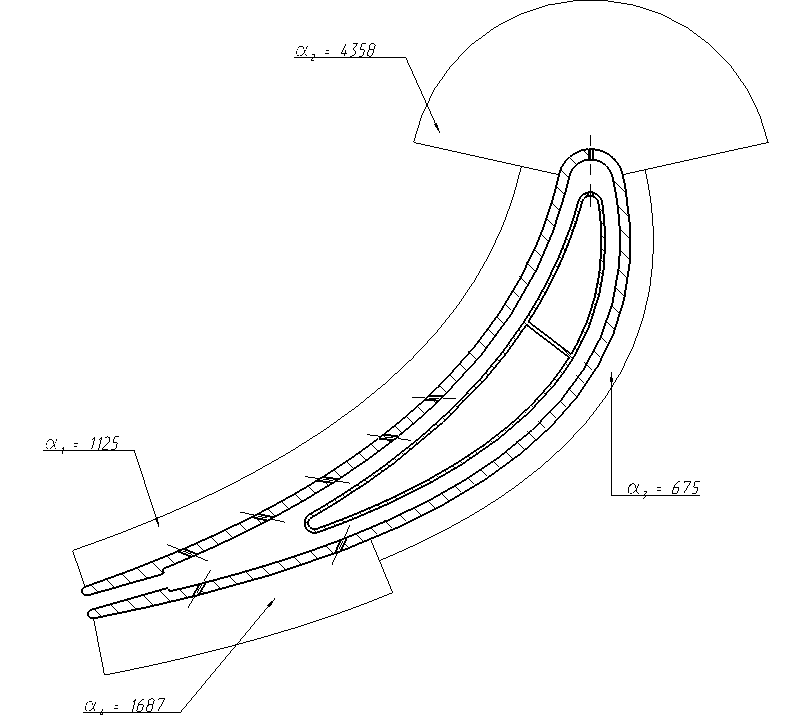
\includegraphics[scale=0.6]{no_spline}
    	\caption{Дискретное распределение коэффициентов теплоотдачи по профилю лопатки}
    \end{figure}

    \begin{figure}[H]
        \centering
        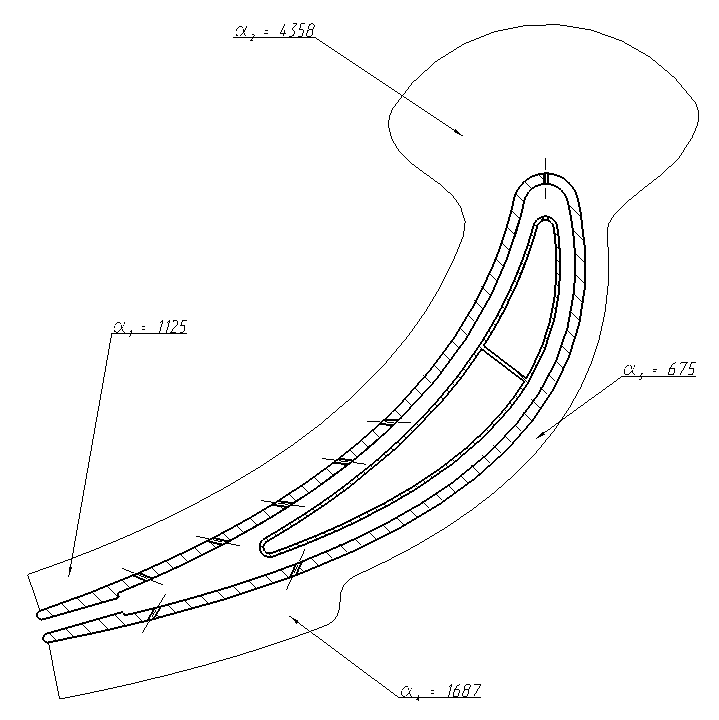
\includegraphics[scale=0.6]{spline}
        \caption{Непрерывное распределение коэффициентов теплоотдачи по профилю лопатки}
    \end{figure}

	\item Уравнение теплообмена между охлаждающим воздухом и газом имеет вид:
		$$
			\frac{d\theta}{dx} = \frac{
				2
			}{
				G_в C_{p \/\ в}
			} \frac{
				k_x
			}{
				\alpha_г
			} \left( 
				T_{пл}^* - \theta
			\right),
		$$
	где $k_x$ - коэффициент теплопередачи, определяемый уравнением
		$$
			k_x = \frac{1}{
				\frac{1}{
					\alpha_{пл}
				} + 
				\frac{1}{
					\alpha_в
				} + 
				\frac{\Delta}{\lambda_м}
			}
		$$
	Численно решая уравнение теплообмена, поулчим распределение параметров по спинке и корыту.
	Распределение параметров газа по спинке:
		\begin{longtable}{|c|c|c|c|c|c|}
		\hline
		\textbf{№} &
		\textbf{$x, \/\ м$} & 
		\textbf{$\alpha_{пл} \/\ Вт/\left(м^2 \cdot К\right)$} & 
		\textbf{$\alpha_в \/\ Вт/\left(м^2 \cdot К\right)$} & 
		\textbf{$\theta_x, \/\ К$} & 
		\textbf{$T_{ст.x}, \/\ К$} 
		\\ \hline
		
			1 & 
			0.000 & 
			4424.3 & 
			1372.6 &
			500.0 & 
			1236.3
			\\\hline
		
			2 & 
			2.705 & 
			666.3 & 
			1417.6 &
			566.0 & 
			862.0
			\\\hline
		
			3 & 
			5.352 & 
			666.3 & 
			1444.7 &
			614.1 & 
			890.7
			\\\hline
		
			4 & 
			7.863 & 
			916.0 & 
			1459.0 &
			643.1 & 
			643.1
			\\\hline
		
			5 & 
			10.253 & 
			732.6 & 
			1462.0 &
			649.4 & 
			711.9
			\\\hline
		
			6 & 
			12.539 & 
			705.2 & 
			1468.9 &
			664.9 & 
			767.6
			\\\hline
		
			7 & 
			14.741 & 
			694.1 & 
			1479.0 &
			688.1 & 
			825.6
			\\\hline
		
			8 & 
			16.882 & 
			688.1 & 
			1489.2 &
			715.0 & 
			866.4
			\\\hline
		
			9 & 
			18.986 & 
			684.3 & 
			1498.5 &
			743.0 & 
			899.4
			\\\hline
		
			10 & 
			21.078 & 
			681.6 & 
			1507.2 &
			771.3 & 
			928.2
			\\\hline
		
			11 & 
			23.184 & 
			732.3 & 
			1511.6 &
			786.3 & 
			835.7
			\\\hline
		
			12 & 
			25.330 & 
			696.8 & 
			1517.0 &
			805.1 & 
			921.1
			\\\hline
		
			13 & 
			27.539 & 
			803.0 & 
			1521.9 &
			824.7 & 
			840.9
			\\\hline
		
			14 & 
			29.834 & 
			705.4 & 
			1525.4 &
			839.1 & 
			931.2
			\\\hline
		
			15 & 
			32.234 & 
			2806.0 & 
			1532.1 &
			863.7 & 
			863.7
			\\\hline
		
			16 & 
			34.757 & 
			1807.5 & 
			1535.4 &
			874.8 & 
			948.1
			\\\hline
		
			17 & 
			37.417 & 
			1754.0 & 
			1545.6 &
			911.1 & 
			1035.4
			\\\hline
		
			18 & 
			40.227 & 
			1863.9 & 
			1549.4 &
			925.4 & 
			958.8
			\\\hline
		
			19 & 
			43.198 & 
			4267.9 & 
			1556.3 &
			951.4 & 
			951.4
			\\\hline
		
			20 & 
			46.339 & 
			1890.8 & 
			1558.3 &
			957.7 & 
			975.3
			\\\hline
		
		\end{longtable}

	Распределение параметров газа по корыту:
		\begin{longtable}{|c|c|c|c|c|c|}
		\hline
		\textbf{№} &
		\textbf{$x, \/\ 10^{-3} м$} & 
		\textbf{$\alpha_{пл} \/\ Вт/\left(м^2 \cdot К\right)$} & 
		\textbf{$\alpha_в \/\ Вт/\left(м^2 \cdot К\right)$} & 
		\textbf{$\theta_x, \/\ К$} & 
		\textbf{$T_{ст.x}, \/\ К$} 
		\\ \hline
		
			1 & 
			0.000 & 
			4424.3 & 
			1372.6 &
			500.0 & 
			1236.3  
			\\\hline
		
			2 & 
			2.577 & 
			1110.5 & 
			1424.7 &
			578.0 & 
			974.8  
			\\\hline
		
			3 & 
			5.198 & 
			1417.0 & 
			1444.2 &
			613.2 & 
			613.2  
			\\\hline
		
			4 & 
			7.731 & 
			1208.9 & 
			1450.8 &
			626.4 & 
			724.9  
			\\\hline
		
			5 & 
			10.179 & 
			1169.9 & 
			1463.9 &
			653.5 & 
			818.5  
			\\\hline
		
			6 & 
			12.550 & 
			1153.5 & 
			1480.5 &
			691.5 & 
			890.2  
			\\\hline
		
			7 & 
			14.848 & 
			1144.4 & 
			1495.0 &
			732.5 & 
			940.2  
			\\\hline
		
			8 & 
			17.081 & 
			1138.6 & 
			1507.7 &
			772.9 & 
			979.8  
			\\\hline
		
			9 & 
			19.256 & 
			1346.4 & 
			1512.6 &
			789.4 & 
			797.3  
			\\\hline
		
			10 & 
			21.380 & 
			1210.1 & 
			1515.3 &
			798.8 & 
			856.7  
			\\\hline
		
			11 & 
			23.463 & 
			1177.9 & 
			1519.9 &
			817.0 & 
			916.0  
			\\\hline
		
			12 & 
			25.514 & 
			1162.8 & 
			1526.5 &
			843.3 & 
			964.8  
			\\\hline
		
			13 & 
			27.541 & 
			1153.8 & 
			1534.8 &
			872.7 & 
			1002.0  
			\\\hline
		
			14 & 
			29.555 & 
			1147.7 & 
			1543.4 &
			902.8 & 
			1033.2  
			\\\hline
		
			15 & 
			31.566 & 
			1396.6 & 
			1545.3 &
			910.0 & 
			910.0  
			\\\hline
		
			16 & 
			33.583 & 
			1250.2 & 
			1546.2 &
			913.3 & 
			932.9  
			\\\hline
		
			17 & 
			35.616 & 
			1207.3 & 
			1549.2 &
			924.8 & 
			956.3  
			\\\hline
		
			18 & 
			37.676 & 
			1574.0 & 
			1551.9 &
			934.8 & 
			934.8  
			\\\hline
		
			19 & 
			39.772 & 
			1266.7 & 
			1553.0 &
			939.2 & 
			950.4  
			\\\hline
		
			20 & 
			41.912 & 
			1216.6 & 
			1557.3 &
			954.5 & 
			974.8  
			\\\hline
			
		\end{longtable}

\end{enumerate}

Распределение температур газа, воздуха и металла по профилю лопатки показано на рис. 6.
\begin{figure}[H]
    \centering
	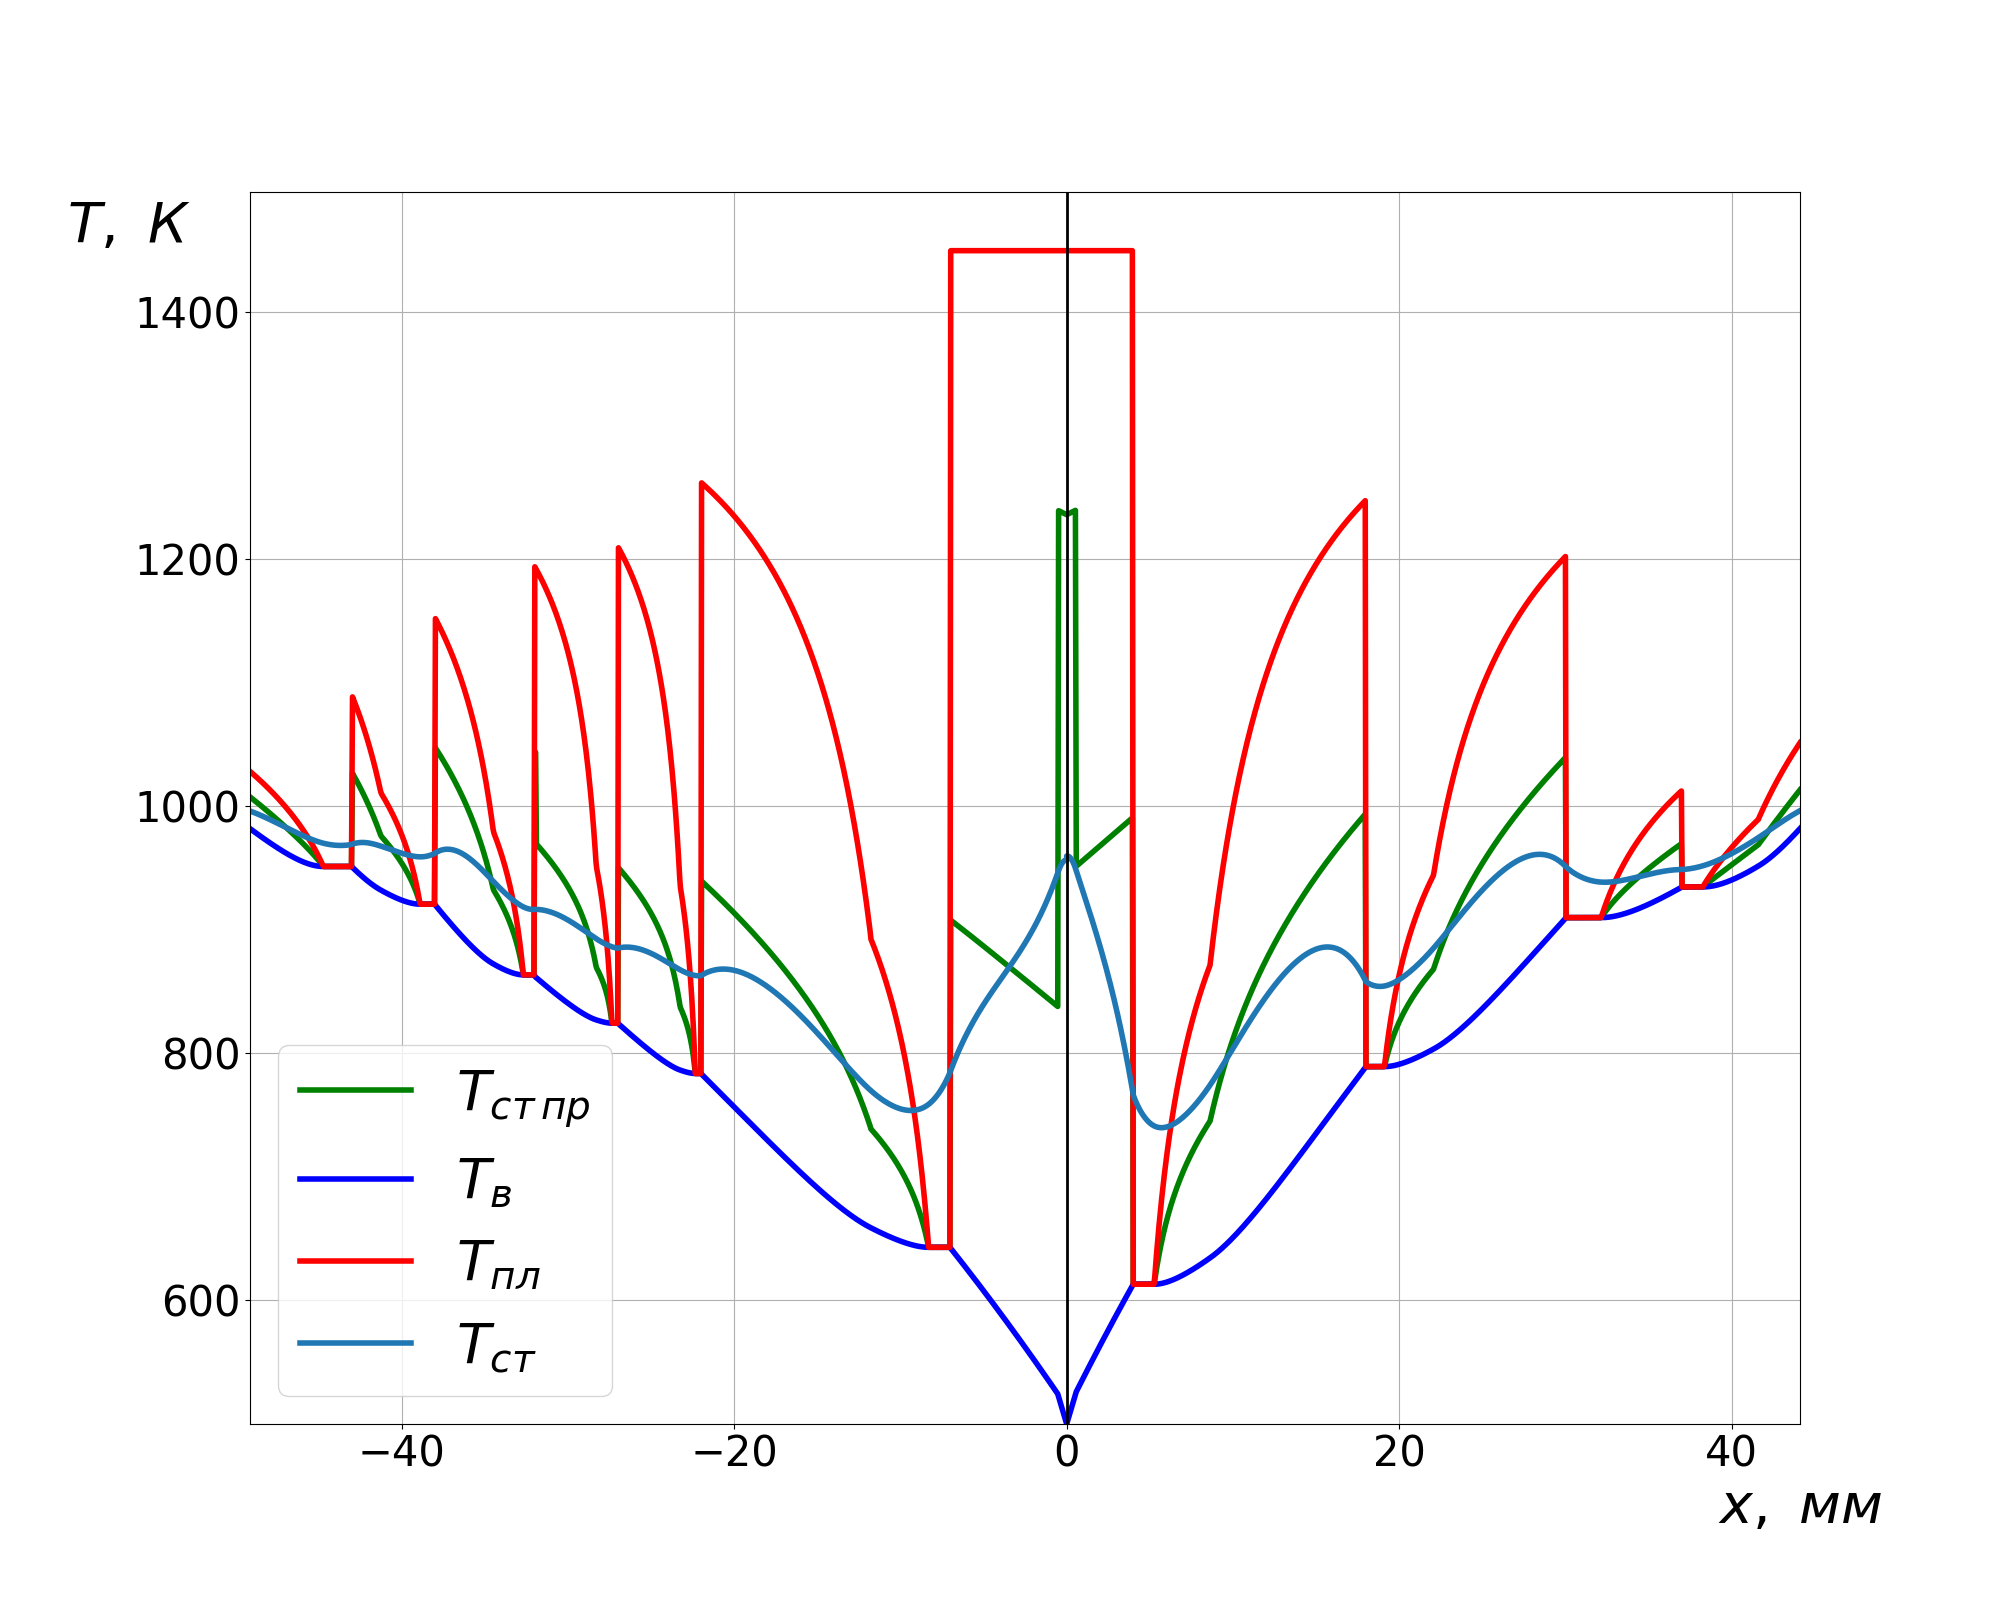
\includegraphics[scale=0.8]{cooling_2_t}
	\caption{Распределение температур газа, воздуха и металла}
\end{figure}

Также был проанализирован вариант без выдува воздуха в лобовой точке (рис. 7). Однако отсутствие выдува в лобовой
точке приводит к сильному перегреву с возможным прогарание профиля лопатки.
\begin{figure}[H]
    \centering
	\includegraphics[scale=0.8]{cooling_2_t_hot}
	\caption{Распределение температур газа, воздуха и металла (без выдува в лобовой кромке)}
\end{figure}

Таким образом, из расчета следует, что ни в одной точке температура материала лопатки не превышает 1100 К (максимальная температура
равна 1081 К), что в случае равномерного поля температур перед сопловыми лопатками обеспечивает достаточную прочность лопаток [1].
Однако основной причиной выхода из строя сопловых лопаток является не температурная деформация, а коррозия.
Для защиты от воздействия агрессивной среды сопловые лопатки покрываются защитным керамическим покрытием на основе
$Zr0_2$ с металлической подложкой на основе $Ni-Cr-Al-Y$. Такой состав покрытия обеспечивает его хорошую адгезию к
основному материалу лопатки и предотвращает его от растрескивания под действием термоциклических нагрузок.
Побочным эффектом применения данного покрытия является снижение температуры основного материала лопатки на 50-60 К
вследствие крайне низкой теплопроводности керамического слоя покрытия.


\end{document}
